\begin{frame}{PC Pitstop's \$1,000 EULA Experiment}
\begin{itemize}
    \item In 2005, PC Pitstop added a hidden clause in its EULA:
    \begin{quote}
        “If you’re reading this and contact us, you may receive money.”
    \end{quote}
    \item Over \textbf{3,000 downloads} later, only \textbf{1 person} noticed—and won \textbf{\$1,000}.
    \item Purpose: Show that users rarely read EULAs.
\end{itemize}

\vspace{0.3cm}
\textit{Proof: Even with an incentive, almost no one reads license agreements.\cite{MONEY}}
\end{frame}

\begin{frame}{Tumblr: Telling It Like It Is}

Tumblr humanizes legal content — a reminder that \textit{Terms of Service don’t have to be soulless}.
    \begin{columns}[c]
    \column{.8\textwidth}
    \begin{figure}
        \centering
        
\includegraphics[width=\textwidth]{images/kids.png}
        \label{fig:kids}
    \end{figure}  
    \begin{figure}
        \centering
        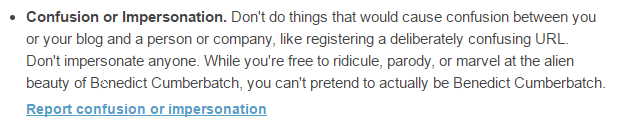
\includegraphics[width=\textwidth]{images/impersonate.png}
        \label{fig:impersonate}
    \end{figure}   
    \column{.2\textwidth}
    \centering
    \begin{figure}
        \centering
        
\includegraphics[width=\textwidth]{images/benedict.jpg}
        \label{fig:benedict}
    \end{figure}    
\end{columns}
\end{frame}

\begin{frame}{Tumblr: Telling It Like It Is}

Tumblr humanizes legal content — a reminder that \textit{Terms of Service don’t have to be soulless}\cite{TUMBLR}.
     \begin{figure}
        \centering
        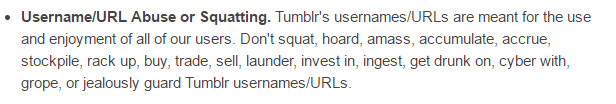
\includegraphics[width=\textwidth]{images/username.png}
        \label{fig:username}
    \end{figure}     
     \begin{figure}
        \centering
        
\includegraphics[width=\textwidth]{images/affirmation.png}
        \label{fig:affirmation}
    \end{figure}     
\end{frame}